%
%  ASMR
%
%  Created by Martell on 2012-04-02.
%  Copyright (c) 2012 UBC Fisheries Centre. All rights reserved.
%
\documentclass{beamer}
%\usetheme{Madrid} % My favorite!
%\usetheme{PaloAlto}
\usetheme{Goettingen}
%\usetheme{Hannover}
%\usetheme{Boadilla} % Pretty neat, soft color.
%\usetheme{default}
%\usetheme{Warsaw}
%\usetheme{Bergen} % This template has nagivation on the left
%\usetheme{Frankfurt} % Similar to the default 
%with an extra region at the top.
%\usecolortheme{seahorse} % Simple and clean template
%\usecolortheme{beaver}
%\usetheme{Darmstadt} % not so good
% Uncomment the following line if you want %
% page numbers and using Warsaw theme%
% \setbeamertemplate{footline}[page number]
%\setbeamercovered{transparent}
\setbeamercovered{invisible}
% To remove the navigation symbols from 
% the bottom of slides%
\setbeamertemplate{navigation symbols}{} 
%
\usepackage{color}
\usepackage{graphicx}
%\usepackage{bm}         % For typesetting bold math (not \mathbold)
%\logo{\includegraphics[height=0.6cm]{yourlogo.eps}}
%

\definecolor{bottomcolour}{rgb}{0.32,0.3,0.38}
\definecolor{middlecolour}{rgb}{0.08,0.08,0.16}
\setbeamerfont{title}{size=\Huge}
\setbeamercolor{structure}{fg=white}
\setbeamertemplate{frametitle}[default][center]

\setbeamercolor{normal text}{bg=black, fg=white}
\setbeamertemplate{background canvas}[vertical shading]
[bottom=bottomcolour, middle=middlecolour, top=black]

\setbeamertemplate{itemize item}{\lower3pt\hbox{\Large\textbullet}}
\setbeamerfont{frametitle}{size=\huge}


\title[Short title of the talk]{Trends and Status of the Little Colorado River population of Humpback Chub: 1989-2011}
\author{Scott Vanderkooi on behalf of Steven Martell}
\institute[UBC]
{
University of British Columbia \\
\medskip
{\emph{s.martell@mail.ubc.ca}}
}
\date{\today}
% \today will show current date. 
% Alternatively, you can specify a date.
%
\begin{document}
%
\begin{frame}
\titlepage
\end{frame}
%
\begin{frame}[t]\frametitle{Outline}
	\tableofcontents
\end{frame}
%
\section[Introduction]{Introduction to ASMR} % (fold)
\label{sec:introduction}
\begin{frame}[t]\frametitle{Introduction to ASMR}
	Mark-recapture information between 1989 and 2011 is used to estimate the abundance and recruitment of Humpback Chub (HBC).\\
	\medskip
	Catch-at-length data are transformed into catch-at-age data using length-age relationship developed from a bioenergetics model.\\
	\medskip
	The unmarked population is reconstructed using Virtual Population Analysis (VPA) with and assumed value of natural mortality rate.\\
	\medskip
	The fate of marked individuals is tracked using an age-structured model, and the capture-recapture probability is assumed to be a Poisson sampling process.\\
\end{frame}
%
\begin{frame}[t]\frametitle{ASMR-3 Analytical details}
	Age Structure Mark Recapture (ASMR-3)\\
	\only<1>{
	\begin{footnotesize}
	\begin{align}
		&\mbox{Data: Marks \& Recaptures} & m_{t,a}, r_{t,a}\\
		&\mbox{Estimate unmarked numbers} & \Theta = \hat{U}_{t=2012,a=2:14} \\
		&\mbox{Survival rate} & S_a =\exp(-M l_\infty/l_a) \\
		&\mbox{Unmarked animals} & \hat{U}_{t,a} = \frac{\hat{U}{t+1,a+1}}{S_a} + m_{t,a}\\
		&\mbox{Marked animals} & \hat{M}_{a+1,t+1} =S_a(\hat{M}_{t,a} +m_{t,a})\\
		&\mbox{Predicted new marks} & \hat{m}_{t,a}=\hat{p}_{t,a}\hat{U}_{t,a}\\
		&\mbox{Predicted recaps} & \hat{r}_{t,a}=\hat{p}_{t,a}\hat{M}_{t,a}\\
		&\mbox{Capture probability} & \hat{p}_{t,a} =
		 \frac{m_{t,a}+r_{t,a}}{\hat{U}_{t,a}+\hat{M}_{t,a}}\\
		&\mbox{Negative log likelihood} & \ell_{t,a}=
		(-\hat{m}_{t,a}+{m}_{t,a}\ln(\hat{m}_{t,a})) \nonumber\\
		& &+(-\hat{r}_{t,a}+{r}_{t,a}\ln(\hat{r}_{t,a}))
	\end{align}
	\end{footnotesize}
	}
	\onslide<2>{
	\textbf{\underline{Assumptions}}:\\
	\begin{itemize}
		\item Natural mortality is a function of length.
		\item Natural mortality is constant over time.
		\item Marked \& unmarked fish have same capture probablility \& survival.
		\item Observation error only.
		\item Growth is time invariant. 
		\item Age is a function of length (slicing).
		\item \underline{Walters \& Martell are never wrong! }
	\end{itemize}
	}
\end{frame}
% section introduction (end)
%
%
\section[Input data]{Input data summary} % (fold)
\label{sec:input_data_summary}
\begin{frame}[t]\frametitle{Marks released}
	\only<1>
	{
	\begin{figure}[htbp]
		\centering
			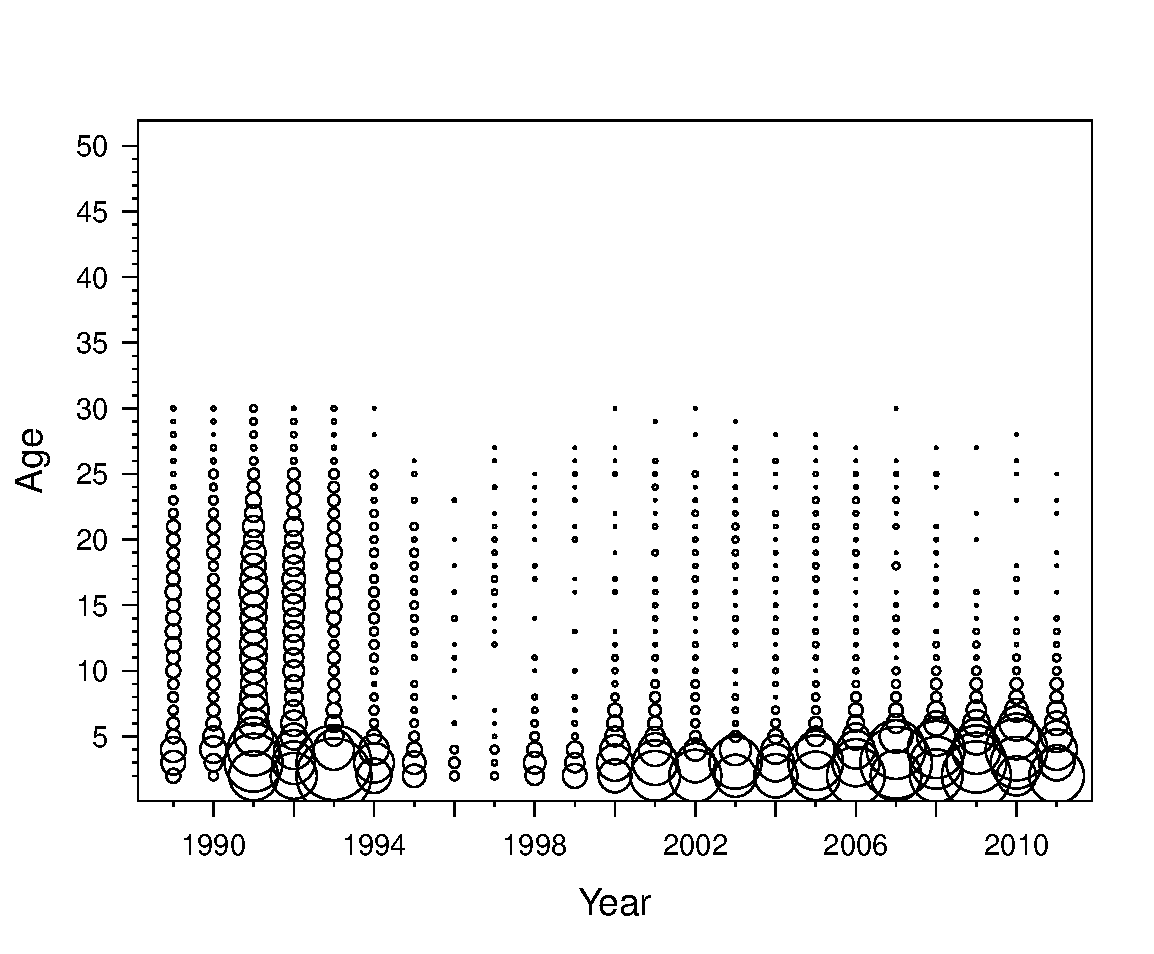
\includegraphics[height=2.4in]{../../FIGS/ASMR/fig:mta.pdf}
		\caption{Number of marks released by age-year. Area of bubble is proportional to the number of marks released.}
		\label{fig:FIGS_ASMR_fig:mta}
	\end{figure}
	
	}
\end{frame}
%
\begin{frame}[t]\frametitle{Marks recaptured}
	\only<1>
	{
		\begin{figure}[htbp]
			\centering
				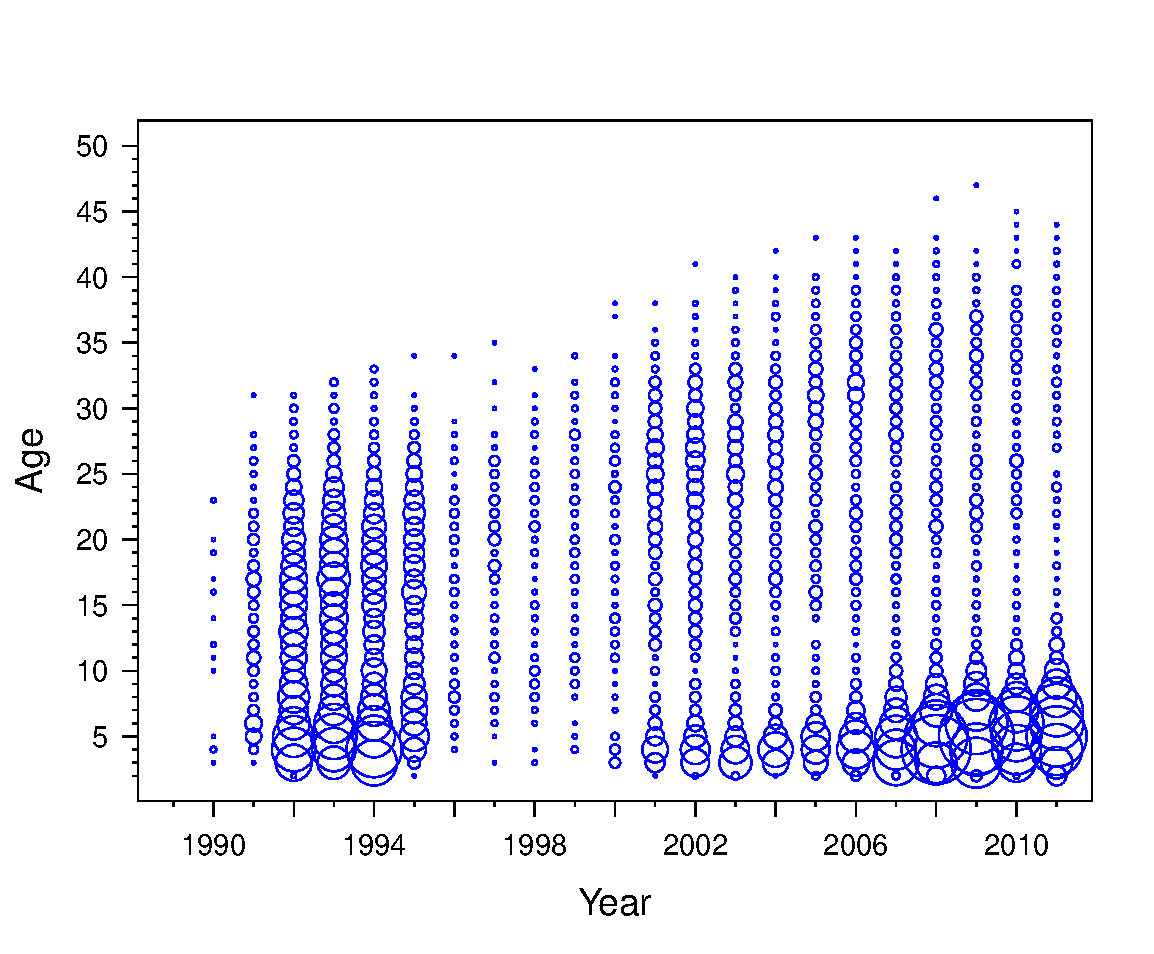
\includegraphics[height=2.4in]{../../FIGS/ASMR/fig:rta.pdf}
			\caption{Number of marks recaptured by age-year. Area of bubble is proportional to the number of marks released.}
			\label{fig:FIGS_ASMR_fig:rta}
		\end{figure}
	}
	\only<2>{
		\begin{figure}[htbp]
			\centering
				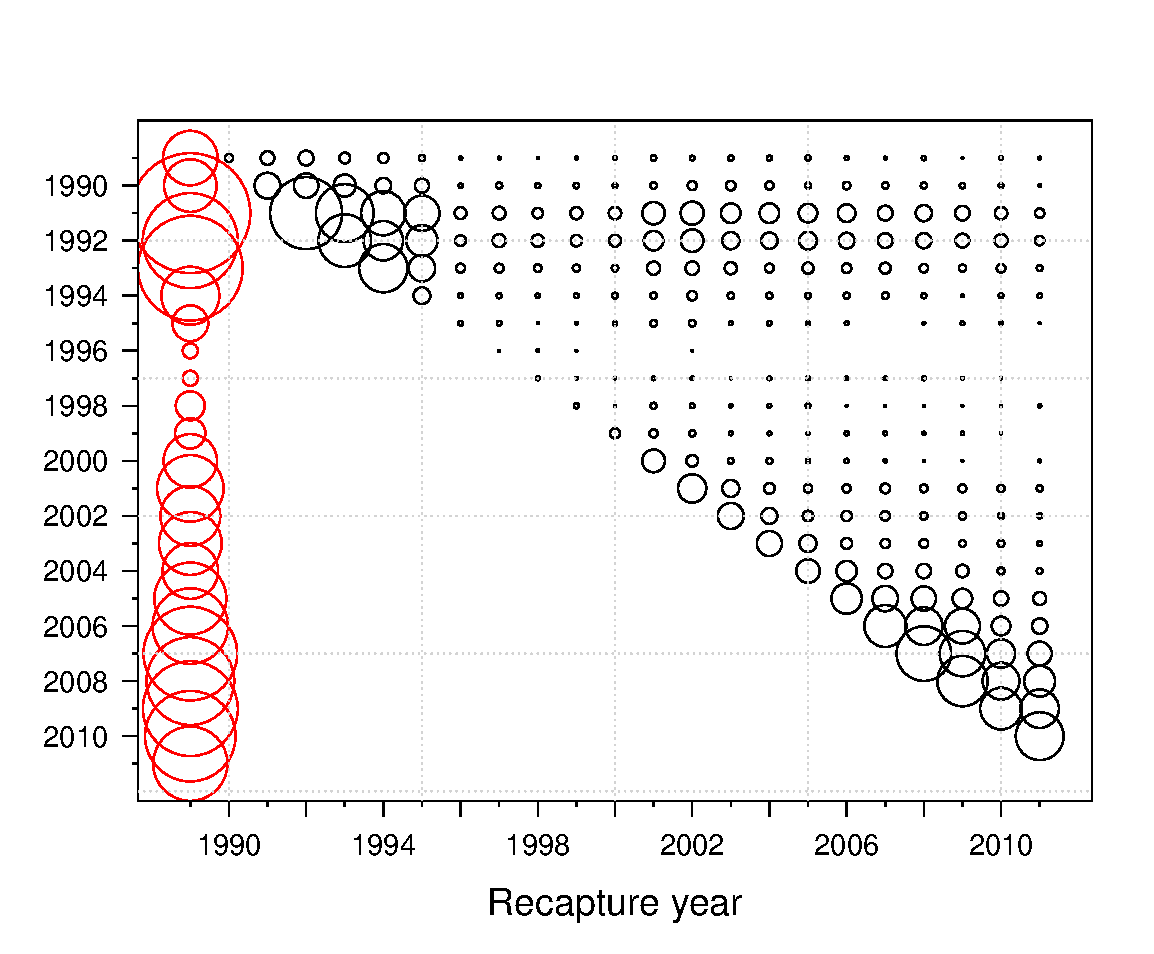
\includegraphics[height=2.4in]{../../FIGS/ASMR/fig:cmr.pdf}
			\caption{Tags released each year (red circles) and number recaptured by tag-year (row of black circles).}
			\label{fig:FIGS_ASMR_fig:cmr}
		\end{figure}
		
	}
\end{frame}
%
% section input_data_summary (end)
%
\section[Results]{Results} % (fold)
\label{sec:results}
\subsection[Abundance]{Abundance & Recruitment} % (fold)
\label{sub:abundance_recruitment}
\begin{frame}[t]\frametitle{Age-4+ abundance}
	\begin{figure}[htbp]
		\centering
			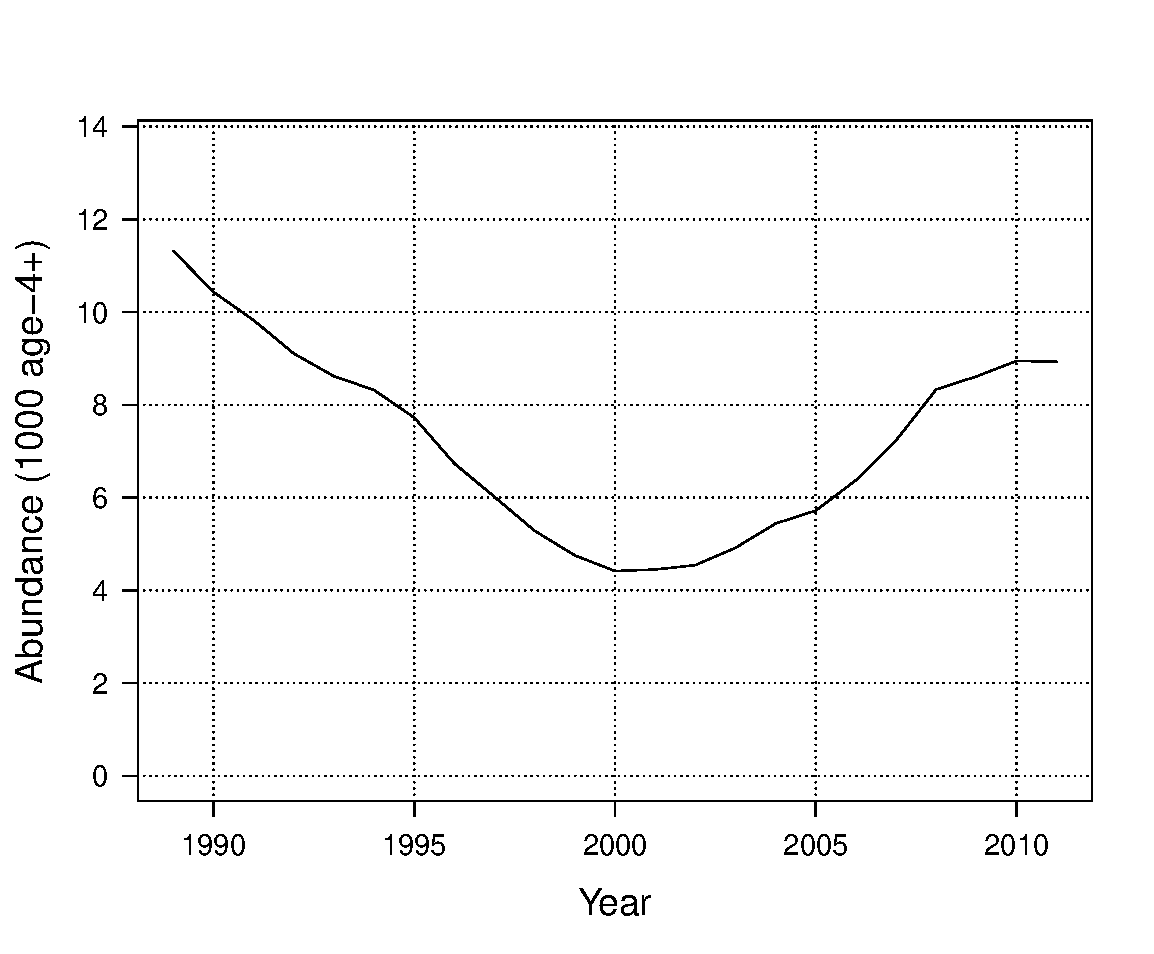
\includegraphics[height=2.4in]{../../FIGS/ASMR/fig:nt4.pdf}
		\caption{Maximum likelihood estimates of age-4+ abundance.}
		\label{fig:FIGS_ASMR_fig:nt4}
	\end{figure}
\end{frame}
%
\begin{frame}[t]\frametitle{Age-2 Recruits}
	\begin{figure}[htbp]
		\centering
			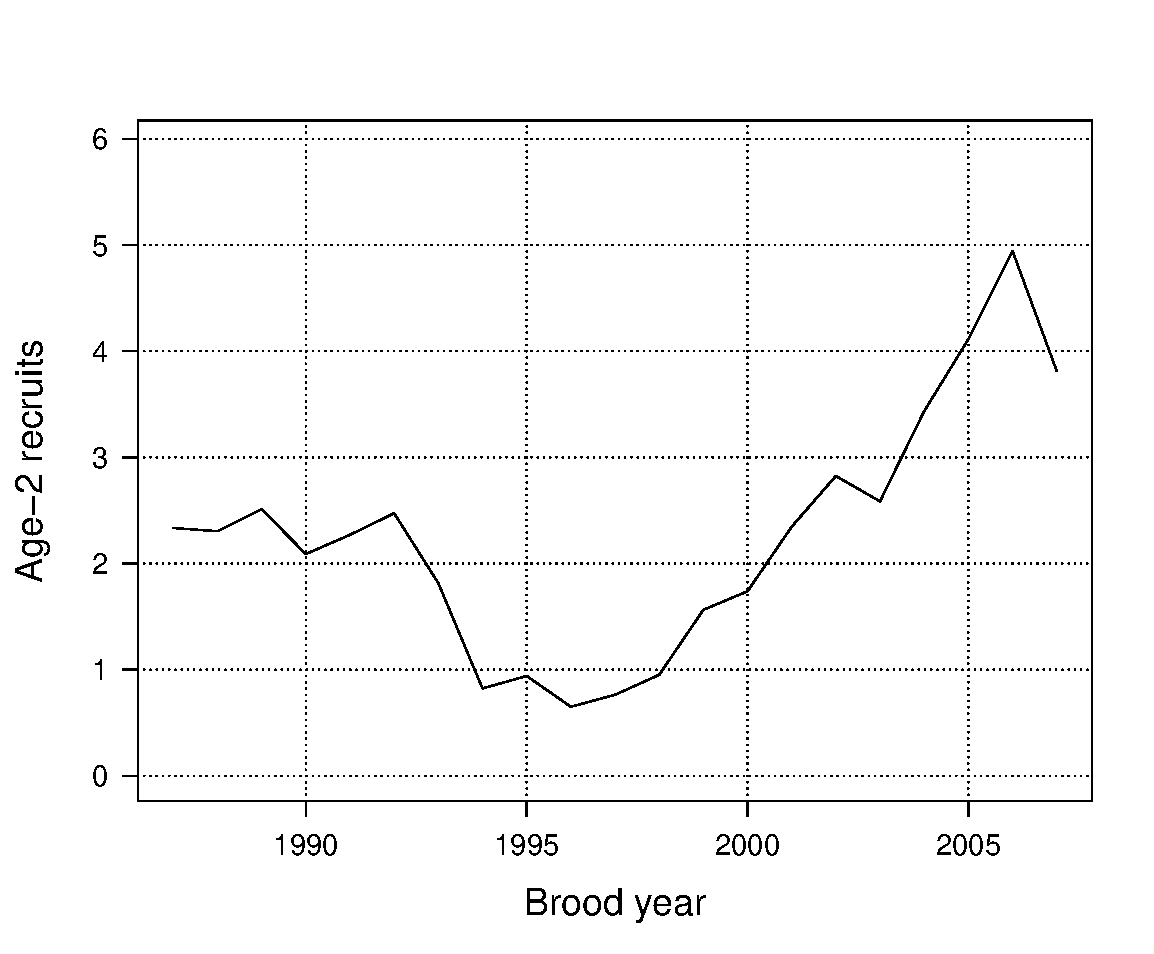
\includegraphics[height=2.4in]{../../FIGS/ASMR/fig:rt.pdf}
		\caption{Maximum likelihood estimates of age-2 recruits.}
		\label{fig:FIGS_ASMR_fig:rt}
	\end{figure}
\end{frame}
%
\begin{frame}[t]\frametitle{Capture probability}
	\begin{figure}[htbp]
		\centering
			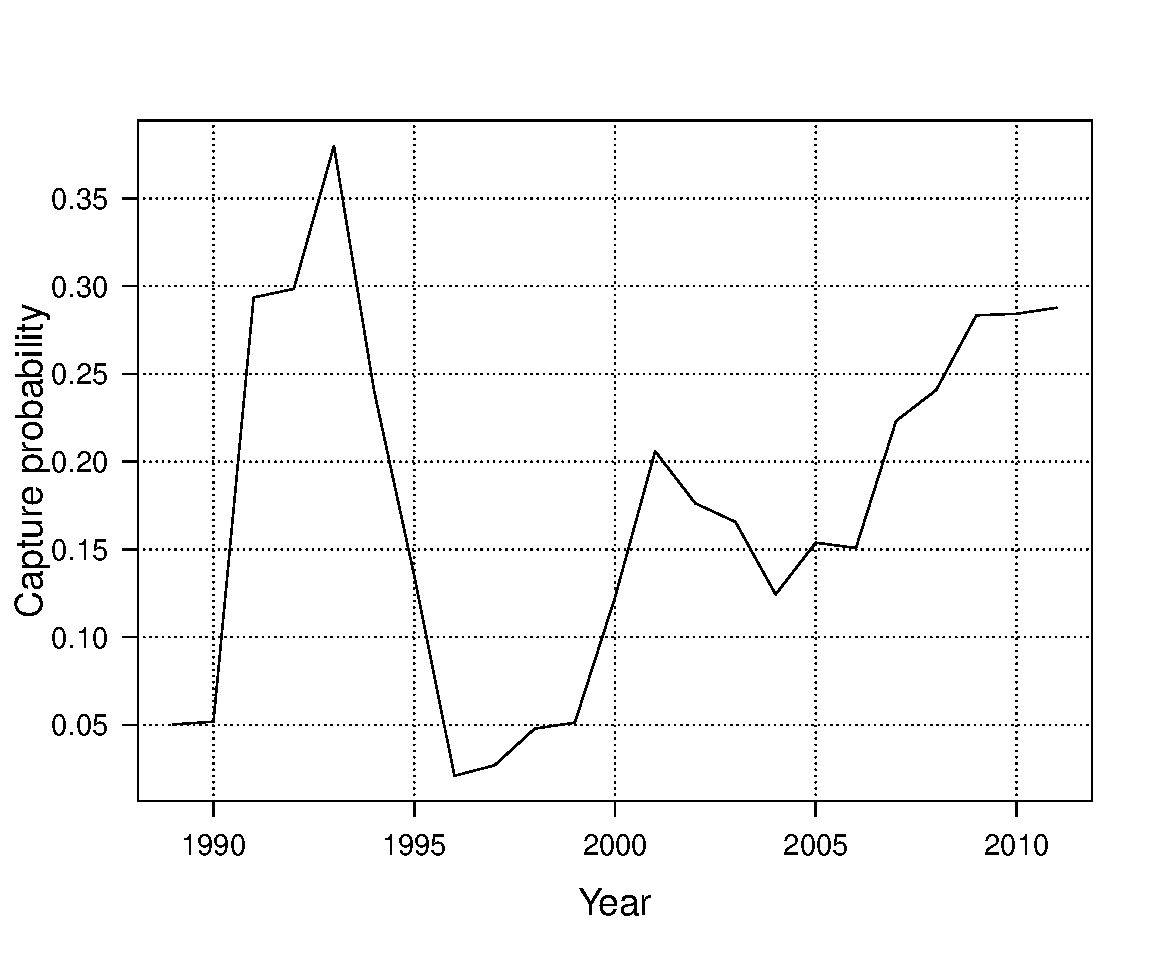
\includegraphics[height=2.4in]{../../FIGS/ASMR/fig:pt.pdf}
		\caption{Maximum likelihood estimates of annual capture probability.}
		\label{fig:FIGS_ASMR_fig:pt}
	\end{figure}
\end{frame}
% subsection abundance_recruitment (end)
%
\subsection{Residuals} % (fold)
\label{sub:residuals}
\begin{frame}[t]\frametitle{Residuals (released marks)}
	\begin{figure}[htbp]
		\centering
			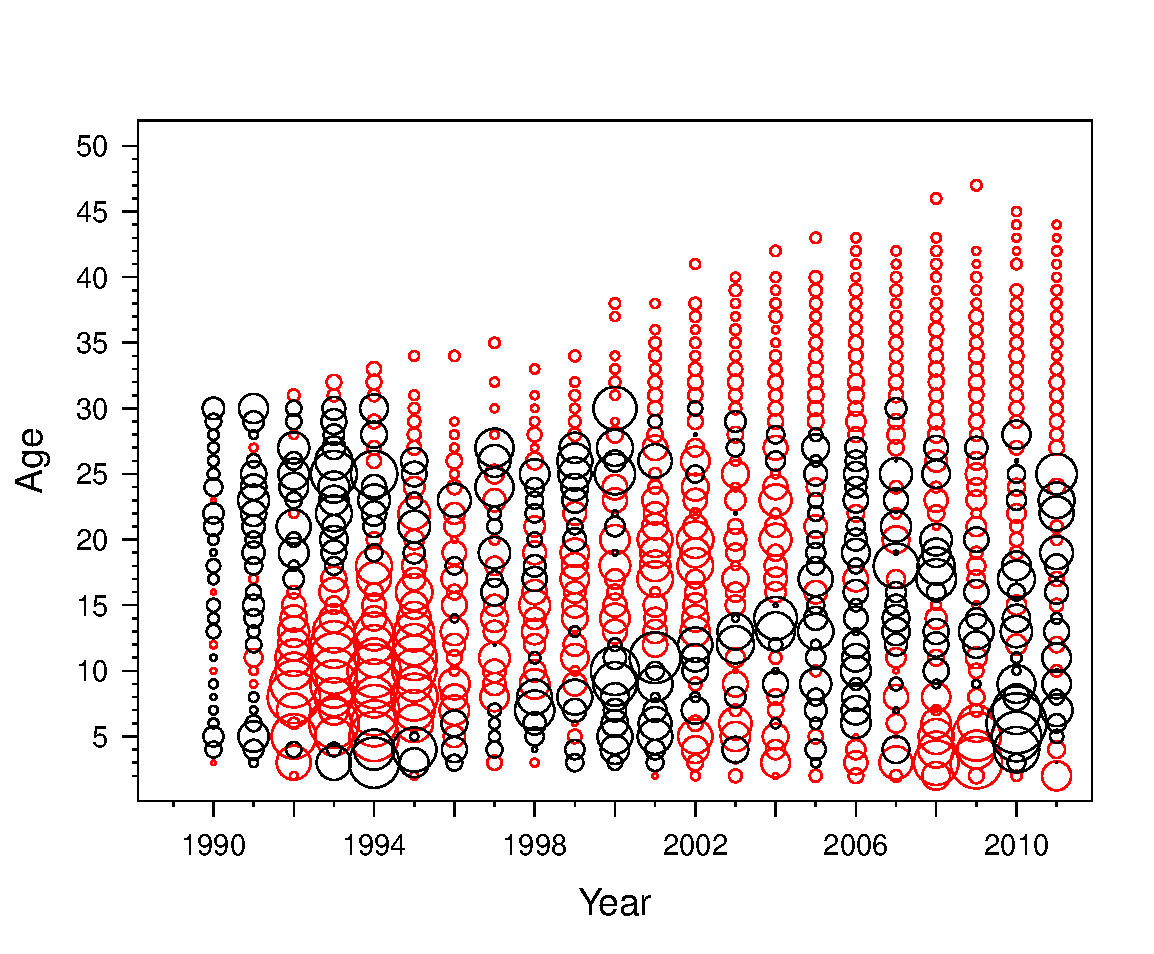
\includegraphics[height=2.4in]{../../FIGS/ASMR/fig:epsilon.pdf}
		\caption{Pearson residuals (observed - expected) for new marks released (black=positive).}
		\label{fig:FIGS_ASMR_fig:epsilon}
	\end{figure}
\end{frame}
\begin{frame}[t]\frametitle{Residuals (recaptured marks)}
	\begin{figure}[htbp]
		\centering
			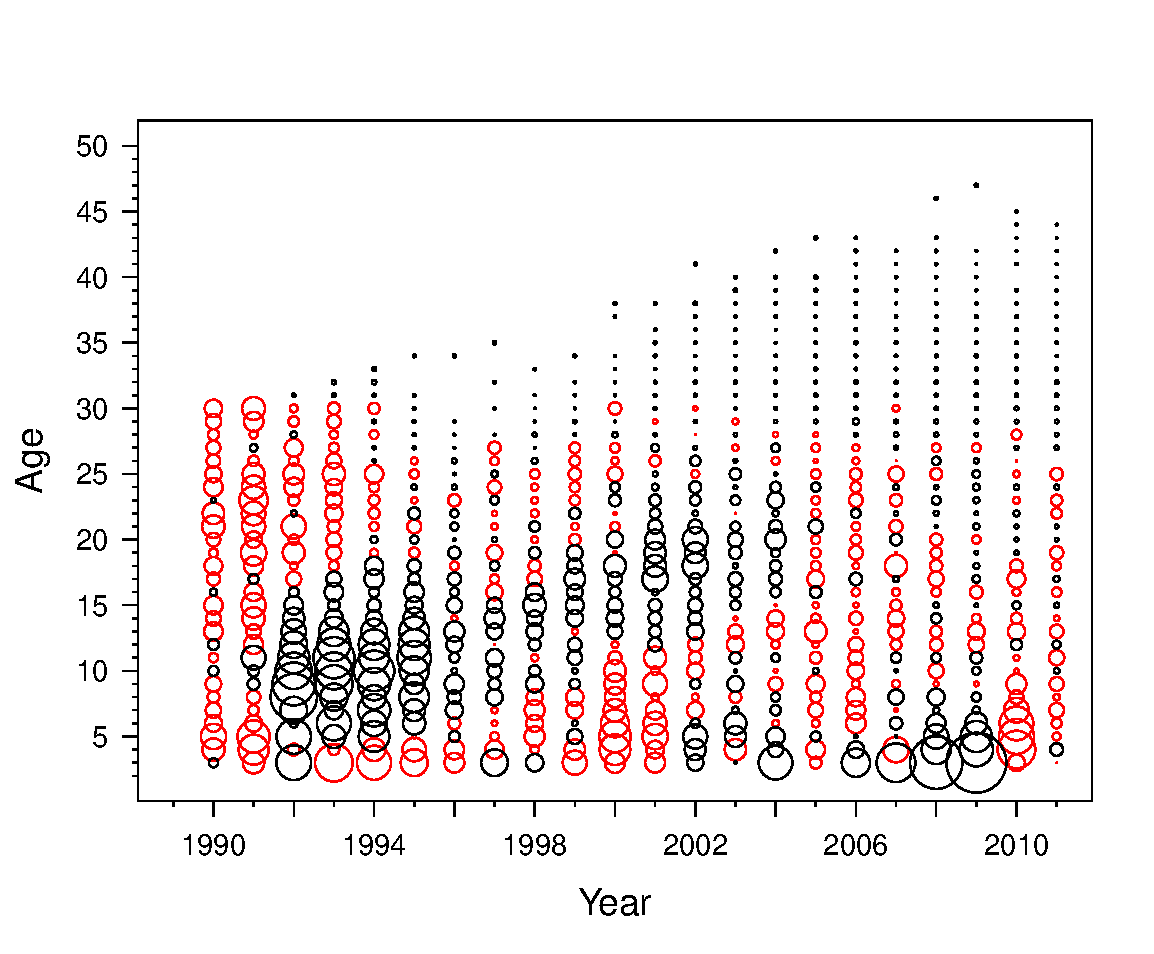
\includegraphics[height=2.4in]{../../FIGS/ASMR/fig:delta.pdf}
		\caption{Pearson residuals (observed - expected) for recaptured marks (black=positive).}
		\label{fig:FIGS_ASMR_fig:delta}
	\end{figure}
\end{frame}
% subsection residuals (end)
%
\subsection[Retrospective]{Retrospecitve Analysis} % (fold)
\label{sub:retrospecitve_analysis}
\begin{frame}[t]\frametitle{Retrospective age-4+ abundance}
	\begin{figure}[htbp]
		\centering
			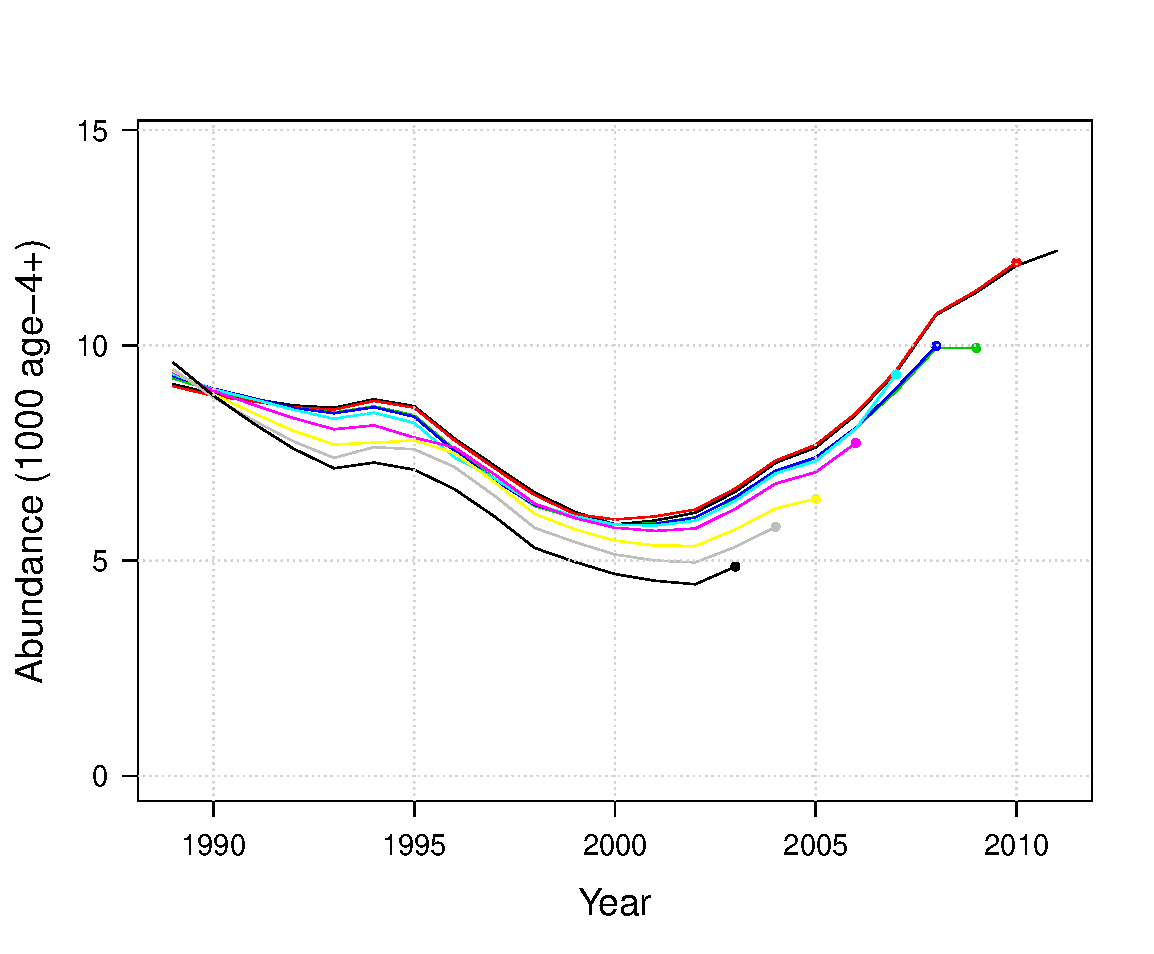
\includegraphics[height=2.4in]{../../FIGS/ASMR/fig:retro_nt4.pdf}
		\caption{Retrospective estimates of age-4+ abundance.}
		\label{fig:FIGS_ASMR_fig:retro_nt4}
	\end{figure}
\end{frame}
%
\begin{frame}[t]\frametitle{Retrospective age-2 recruits}
	\begin{figure}[htbp]
		\centering
			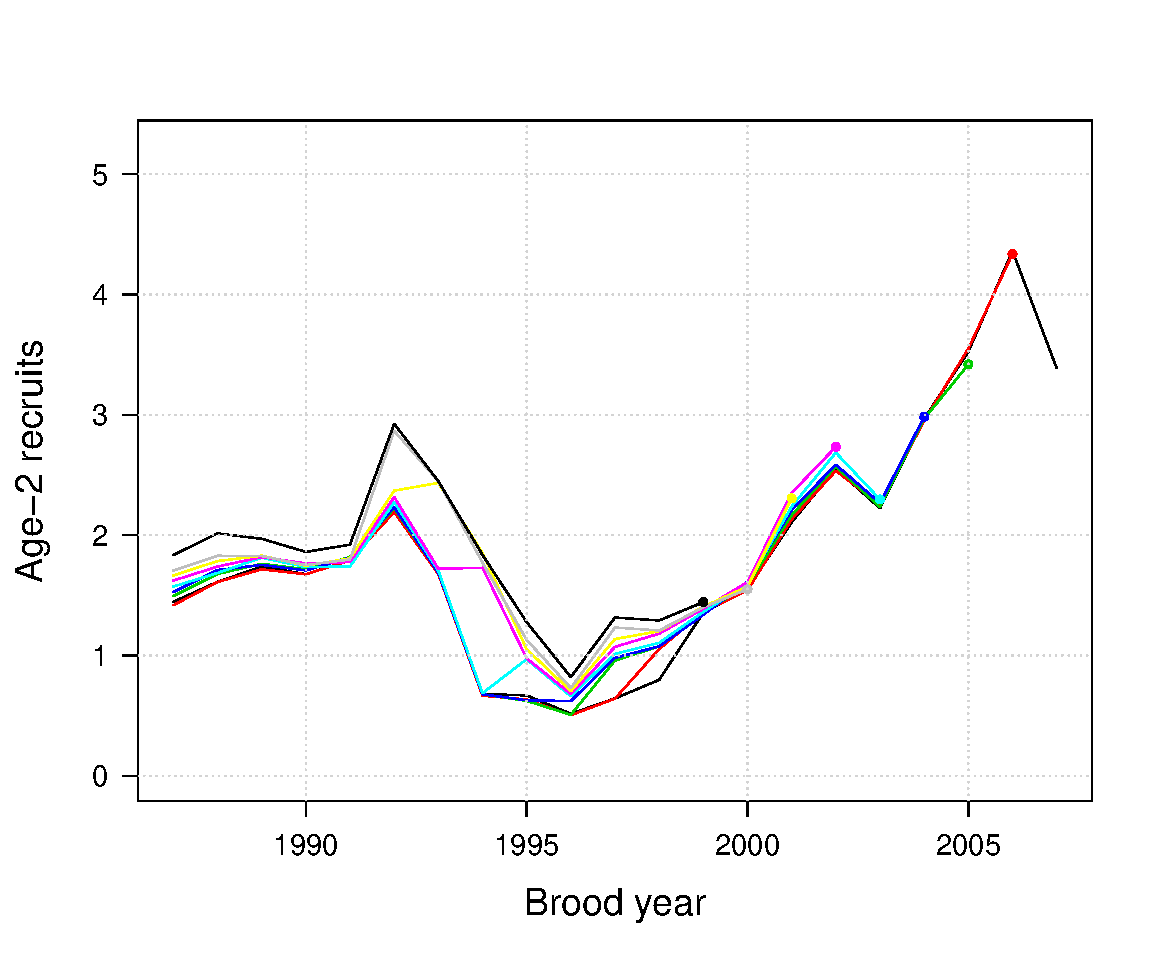
\includegraphics[height=2.4in]{../../FIGS/ASMR/fig:retro_rt.pdf}
		\caption{Retrospective estimates of age-2 recruits.}
		\label{fig:FIGS_ASMR_fig:retro_rt}
	\end{figure}
	
\end{frame}
% subsection retrospecitve_analysis (end)
%
\subsection{Uncertainty} % (fold)
\label{sub:uncertainty}
\begin{frame}[t]\frametitle{Uncertainty: Age-4+ \& Age-2}
	\begin{figure}[htbp]
		\centering
			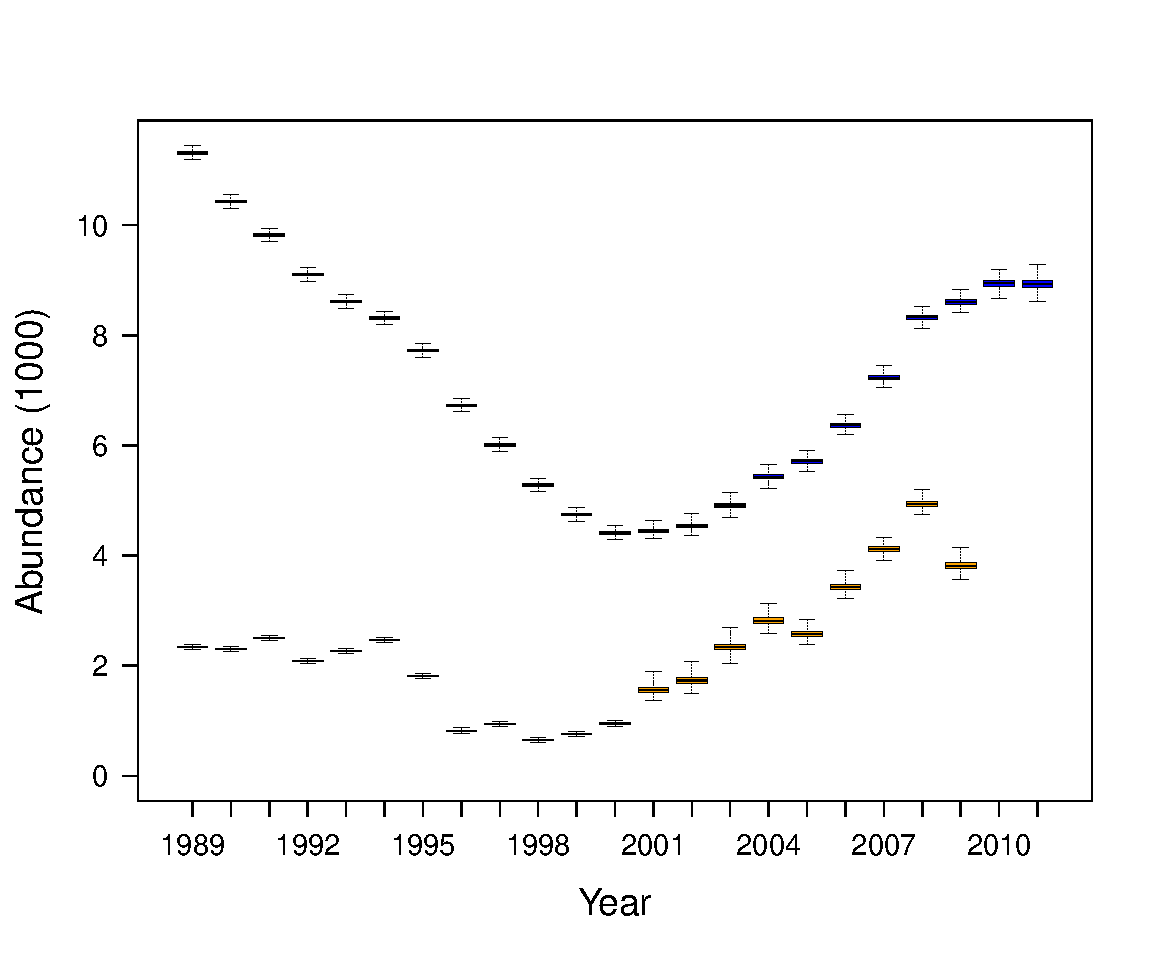
\includegraphics[height=2.4in]{../../FIGS/ASMR/fig:bxplt_Nt4_rt.pdf}
		\caption{Marginal distributions for age-4+ (blue) abundance and age-2 recruits (orange).}
		\label{fig:FIGS_ASMR_fig:bxplt_Nt4_rt}
	\end{figure}
\end{frame}
\begin{frame}[t]\frametitle{Age-4+ abundance in 2011}
	\begin{figure}[htbp]
		\centering
			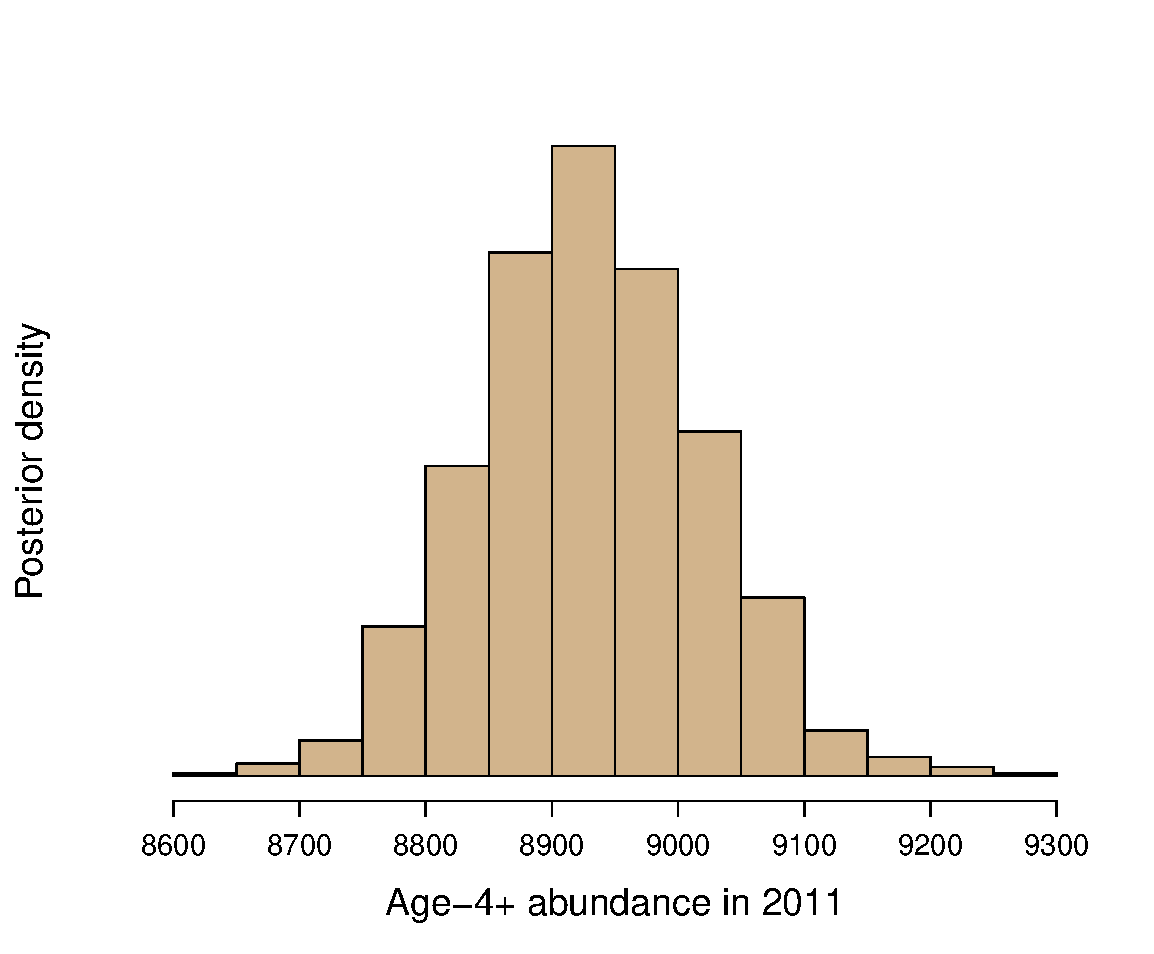
\includegraphics[height=2.4in]{../../FIGS/ASMR/fig:marg_Nt4.pdf}
		\caption{Marginal posterior density for age-4+ abundance in 2011.}
		\label{fig:FIGS_ASMR_fig:marg_Nt4}
	\end{figure}
\end{frame}
% subsection uncertainty (end)
\subsection{Sensitivity to $M$} % (fold)
\label{sub:sensitivity_to_m_}
\begin{frame}[t]\frametitle{Sensitivity to natural mortality ($M$)}
	\only<1>
	{
		\begin{figure}[htbp]
			\centering
				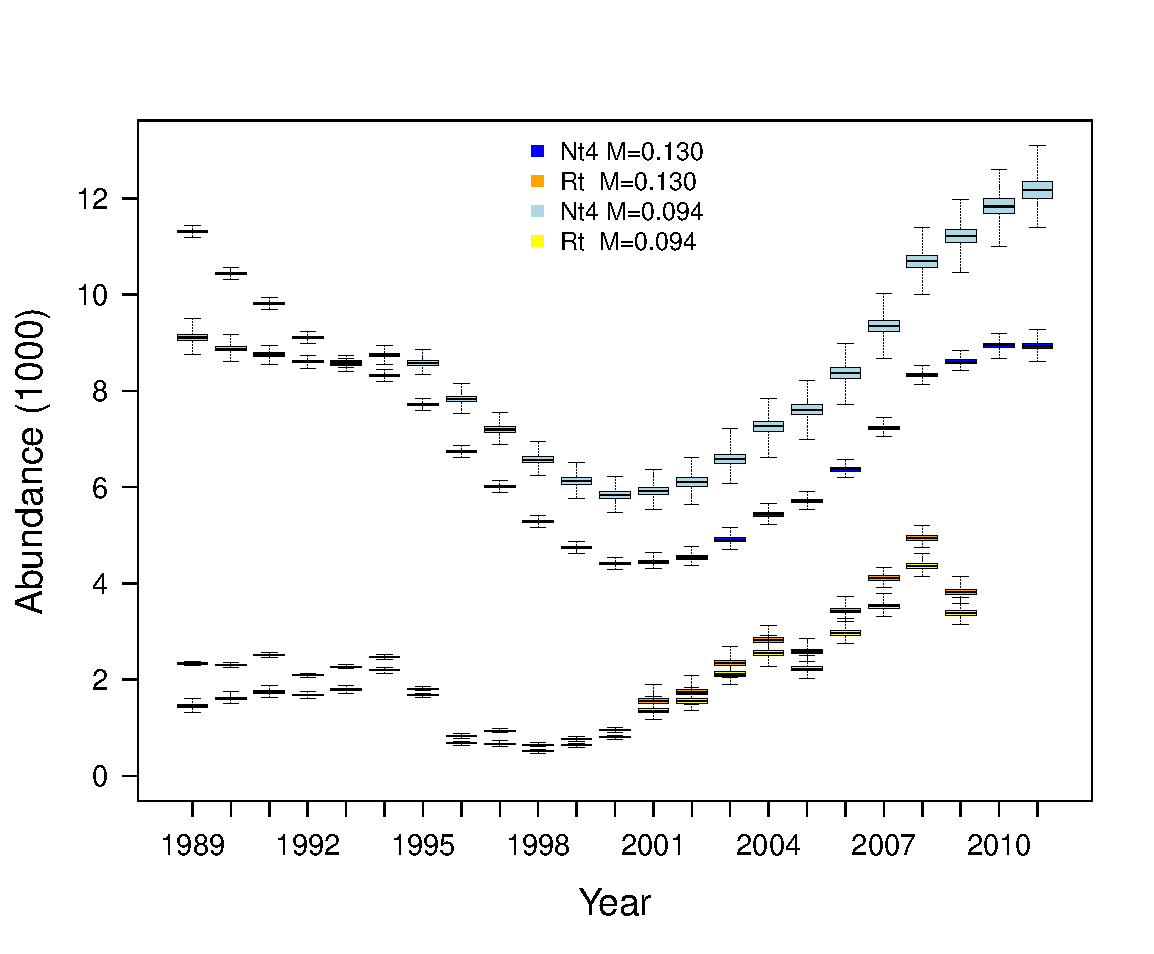
\includegraphics[height=2.4in]{../../FIGS/ASMR/fig:bxplt_Nt4_rt_estM.pdf}
			\caption{Freely estimating natural mortality results in increased estimates of age-4 abundance and fewer age-2 recruits.}
			\label{fig:FIGS_ASMR_fig:bxplt_Nt4_rt_estM}
		\end{figure}
	}
	\only<2>
	{
		\begin{figure}[htbp]
			\centering
				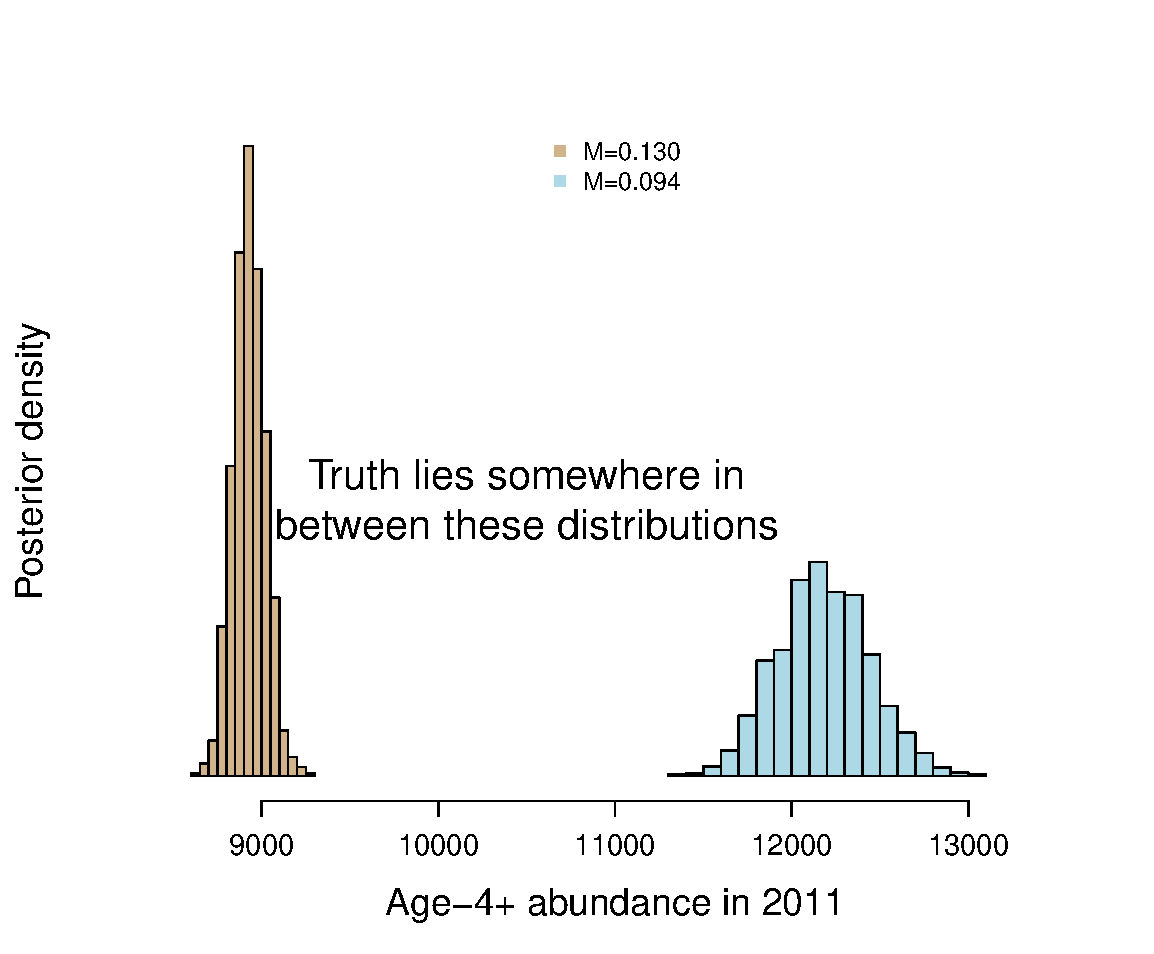
\includegraphics[height=2.4in]{../../FIGS/ASMR/fig:marg_Nt4_estM.pdf}
			\caption{Marginal posterior density for age-4+ abundance in 2011 with M=0.13 (tan) and M=0.094 (light blue).}
			\label{fig:FIGS_ASMR_fig:marg_Nt4_estM}
		\end{figure}
		
	}
\end{frame}
% subsection sensitivity_to_m_ (end)
% section results (end)
\section{Summary} % (fold)
\label{sec:summary}
\begin{frame}[t]\frametitle{Summary}
	Strong residual pattern arising from large number of tags released in 1993-94, and indication of a lower natural mortality rate.\\
	\pause \medskip
	Assuming the asymptotic natural mortality rate of 0.13:\\
	\begin{itemize}
		\item     Median age-4+ in 2011: 8912  (8736, 9095)--95\%CI
		\item     Median age-2 in 2011: 3998  (3814, 4195)--95\%CI
	\end{itemize}
	\pause \medskip
	Freely estimating natural mortality rate ($M=0.094$):\\
	\begin{itemize}
		\item     Median age-4+ in 2011: 12274 (11773, 12812)--95\%CI
		\item     Median age-2 in 2011: 3635  (3463, 3838)--95\%CI
	\end{itemize}
	\pause \medskip
	Uncertainty is grossly under-estimated due to observation error only, and assignment of age from length.
\end{frame}
%
\begin{frame}[t]\frametitle{Acknowledgments}
	\vfill
	Lew Coggins, Carl Walters, Josh Korman and Bill Pine for technical assistance and development of ASMR.\\
	\vfill
	GCMRC Staff: Scott Vanderkooi, Bill Persons, Ted Melis, Glenn Bennett, Mike Yard \& the many other volunteers (some even busting their ass, literally!) who worked in the canyon collecting all of this data.
\end{frame}
% section summary (end)
% End of slides
\end{document}

